% ------------------------------------------------------------------------------
% Este fichero es parte de la plantilla LaTeX para la realización de Proyectos
% Final de Grado, protegido bajo los términos de la licencia GFDL.
% Para más información, la licencia completa viene incluida en el
% fichero fdl-1.3.tex

% Copyright (C) 2012 SPI-FM. Universidad de Cádiz
% ------------------------------------------------------------------------------

El objetivo de esta sección del documento es presentar el plan de pruebas seguido, 
incluyendo los diferentes tipos de pruebas que se han realizado. 

En primer lugar se describe la estrategia de pruebas seguida. Para ello se describe 
el alcance de estas y el procedimiento de pruebas de regresión realizado. 

Otro aspecto tratado es la descripción del entorno que se deberá utilizar para la
realización de las pruebas. Esto incluye los requisitos de software y hardware necesarios. 

Además se incluyen los perfiles y participantes necesarios para llevar a cabo los casos 
de prueba. Esto son los roles desde los que se llevarán a cabo las pruebas.

Por último se documentan las diferentes pruebas realizadas según el tipo al que estas pertenecen.

\section{Estrategia}
Las pruebas llevadas a cabo comprenden toda la funcionalidad del sistema. En cada iteración del ciclo de
vida se realizan pruebas relativas a las funcionalidades comprendidas en la misma. 

Para el diseño de las pruebas se ha tomado un enfoque funcional o de caja negra, centrada en la 
especificación de las funciones, la entrada y salida. La técnica utilizada consiste en definir 
los casos de pruebas a partir de clases de equivalencias:

\begin{enumerate}
\item Identificar las restricciones de formato y contenido de los datos de entrada.
\item A partir de las restricciones identificar las clases de equivalencias. Contemplando tanto 
datos válidos como erróneos.
\item Se identifican y definen los casos de prueba a partir de las clases de equivalencias.
\end{enumerate}

Para asegurar la estabilidad en el resultado de las pruebas realizadas en cada iteración, se ha implementado un mecanismo
que lleve a cabo las pruebas de forma regresiva, ejecutándose todo el conjunto de estas cada vez que una nueva funcionalidad 
del software es desarrollada. 

Además de realizar pruebas funcionales en cada iteración, se han realizado una serie de pruebas no funcionales. 
Esta comprende aquellas que aseguran que se cumplen los requisitos no funcionales.

\section{Entorno de pruebas}
En este punto se define el entorno utilizado para las pruebas, tanto a nivel de software como a nivel de hardware. 

\subsection{Hardware}
Para las pruebas se ha tomado un PC de características medias, en el momento de la realización del proyecto. Este se conforma de:

\begin{description}
\item [CPU:]  Intel Core i5-4460 3.2Ghz 
\item [Disco Duro:] 1TB Western/Seagate
\item [Memoria Ram:] 4GB DDR3 1333 PC3-10600 CL9 Kingston
\item [Placa Base:] Gigabyte GA-H81M-S2H   
\item [Tarjeta gráfica:] 1GB Integrada Intel 
\end {description}

\subsection{Software}
Para las pruebas se ha utilizado un sistema GNU/Linux, instalado y configurado desde una distribución de paquetes 
Debian 8 Jessie. 

\begin{description}
\item [Sistema operativo:] GNU/Linux 
\item [Distribución de paquetes:] Debian Jessie 8
\item [Entorno gráfico:] Xfce 4
\item [Interprete de comando:] Bash 4.3.8
\item [Interprete OMI:] OMI 0.1
\end{description}

\section{Roles}
Las pruebas se han llevado a cabo desde la perspectiva del único rol que interactuará con el sistema correspondiente al usuario que 
normalmente será un programador que hará uso del mismo.

El usuario programador hace uso integro del sistema en función a los programas que desarrolle en el lenguaje. Un único programa, o conjunto finito de estos no 
son suficientes para probar todos los aspectos del sistema. Así aunque las pruebas son llevadas a cabo desde un perfil programador, estas no constituyen programas 
completos con un objetivo específico, sino baterías de pruebas que pretenden probar cada aspecto funcional del sistema. 

\section{Niveles de pruebas}
Las pruebas se presentan en distintos niveles, según el tipo de prueba realizado. Dado la gran cantidad de pruebas estas en su mayoría han sido automatizadas, presentándose
junto al sistema y siendo una característica más del mismo, la cual es recomendable ejecutar tras cada instalación. 

\subsection{Pruebas unitarias}
Son pruebas llevadas a cabo sobre cada artefacto o pieza software producido en cada iteración del ciclo de desarrollo. Estas aseguran la correcta implementación
de las piezas desarrolladas, comprobando que están libre de errores y que cada entrada es procesada correctamente. Además cada caso de prueba se ha estructurado en función 
los tipos de entradas para una mejor organización de las mismas. 
 
Las pruebas unitarias están recogidas en un subsistema de la aplicación que automatizan su ejecución y asegura que son llevadas a cabo de forma regresiva. Este subsistema consiste en
un script bash que se encarga de ejecutar varios script OMI que implementan pruebas unitarias, la salida de la ejecución será comparada con ficheros de texto plano que guardan el resultado correcto de
las mismas. 

A continuación se expone algunos ejemplos de las pruebas unitarias realizadas:

\subsubsection{Asignación de booleanos}
Estos casos de prueba se centran en el operador asignación cuando el elemento asignado es de valor boolenano.

%~ \begin{framed}
	\begin{description}
		\item [Entrada:]\hfill \\
\begin{lstlisting}
 a = true;
\end{lstlisting}
		\item [Descripción:] Asignación sobre la variable $a$ el valor booleano true.
		\item [Salida esperada:] $a$ tiene el valor true.
		\item [Salida obtenida:] $a$ tiene el valor true.
	\end{description} 
%~ \end{framed}
\hfil \\
%~ \begin{framed}
	\begin{description}
		\item [Entrada:] \hfill \\
\begin{lstlisting}
 a = false;
\end{lstlisting}
		\item [Descripción:] Asignación sobre la variable $a$ el valor booleano false.
		\item [Salida esperada:] $b$ tiene el valor false.
		\item [Salida obtenida:] $b$ tiene el valor false.
	\end{description}
%~ \end{framed}
\hfil \\
%~ \begin{framed}
	\begin{description}
		\item [Entrada:] \hfill \\
\begin{lstlisting}
 for (i = 0; i < 10; ++i) 
   a = true;
\end{lstlisting}
		\item [Descripción:] A la variable $a$ se le asigna el valor booleano true en cada iteración del bucle
		\item [Salida esperada:] $a$ tiene el valor true.
		\item [Salida obtenida:] $a$ tiene el valor true.
	\end{description} 
%~ \end{framed}
\hfil \\
%~ \begin{framed}
	\begin{description}
		\item [Entrada:] \hfill \\
\begin{lstlisting}
 a = b = true;
\end{lstlisting}
		\item [Descripción:] A la variable $b$ se le asigna el valor booleano true, el valor de $b$ es asignado a $a$
		\item [Salida esperada:] Tanto $b$ como $a$ tienen el valor true.
		\item [Salida obtenida:] Tanto $b$ como $a$ tienen el valor true.
	\end{description}
%~ \end{framed}
\hfil \\
%~ \begin{framed}
	\begin{description}
		\item [Entrada:] \hfill \\
\begin{lstlisting}
 array[0] = true;
\end{lstlisting}
		\item [Descripción:] A el array $array$ se le asigna en el índice 0 el valor true
		\item [Salida esperada:] $array$ contiene en la para la clave 0 el valor true. Si $array$ no existe es creado.
		\item [Salida obtenida:] $array$ contiene en la para la clave 0 el valor true. Si $array$ no existe es creado.
	\end{description}
%~ \end{framed}
\hfil \\
%~ \begin{framed}
	\begin{description}
		\item [Entrada:] \hfill \\
\begin{lstlisting}
 array[1] = true
\end{lstlisting}
		\item [Descripción:] A el array $array$ se le asigna en el índice 1 el valor false
		\item [Salida esperada:] $array$ contiene en la para la clave 1 el valor false. Si $array$ no existe es creado.
		\item [Salida obtenida:] $array$ contiene en la para la clave 1 el valor false. Si $array$ no existe es creado.
	\end{description}
%~ \end{framed}
\hfil \\
%~ \begin{framed}
	\begin{description}
		\item [Entrada:] \hfill \\
\begin{lstlisting}
 for (i = 0; i < 10; ++i) 
   array[i] = true;
\end{lstlisting}
		\item [Descripción:] A el array $array$ se le asigna el valor true a los índices que van desde 0 a 9.
		\item [Salida esperada:] $array$ contiene en la para las claves del 0 al 9 el valor true. Si $array$ no existe es creado.
		\item [Salida obtenida:] $array$ contiene en la para las claves del 0 al 9 el valor true. Si $array$ no existe es creado.
	\end{description}
%~ \end{framed}
\hfil \\
%~ \begin{framed}
	\begin{description}
		\item [Entrada:] \hfill \\
\begin{lstlisting}
 str = "ABCDEF"; 
 str[0] = false;
\end{lstlisting}
		\item [Descripción:] A la cadena $str$ se le asigna en la posición 0 el valor false.
		\item [Salida esperada:] La cadena $str$ queda con el ínice $0$ con el valor false. La cadena resultante es "BCDEF".
		\item [Salida obtenida:] La cadena $str$ queda con el índice $0$ con el valor false. La cadena resultante es "BCDEF".
	\end{description}
%~ \end{framed}
\hfil \\
%~ \begin{framed}
	\begin{description}
		\item [Entrada:] \hfill \\
\begin{lstlisting}
 str = "ABCDEF"; 
 str[0] = true;
\end{lstlisting}
		\item [Descripción:] A la cadena $str$ se le asigna en la posición 0 el valor true.
		\item [Salida esperada:] La cadena $str$ queda con el índice $0$ con el valor true. La cadena resultante es "1BCDEF".
		\item [Salida obtenida:] La cadena $str$ queda con el índice $0$ con el valor true. La cadena resultante es "1BCDEF".
	\end{description}
%~ \end{framed}
\hfil \\
%~ \begin{framed}
	\begin{description}
		\item [Entrada:] \hfill \\
\begin{lstlisting}
 while (size str) 
   str[0] = false;
\end{lstlisting}
		\item [Descripción:] A la cadena $str$ se le asigna en la posición 0 el valor false, mientras que la cadena sea distinta a la cadena vacía.
		\item [Salida esperada:] La cadena $str$ queda vacía.
		\item [Salida obtenida:] La cadena $str$ queda vacía.
	\end{description}
%~ \end{framed}

%~ \begin{framed}
	\begin{description}
		\item [Entrada:] \hfill \\
\begin{lstlisting}
 a = false; 
 b = &a; 
 a = true; 
\end{lstlisting}
		\item [Descripción:] A $a$ se le asigna el valor false, a $b$ se le asigna una referencia a $a$, a $a$ se le asigna el valor true.
		\item [Salida esperada:] Tanto el valor de $b$ como el de $a$ es true.
		\item [Salida obtenida:] Tanto el valor de $b$ como el de $a$ es true.
	\end{description}
%~ \end{framed}
\hfil \\
%~ \begin{framed}
	\begin{description}
		\item [Entrada:] \hfill \\
\begin{lstlisting}
 true = true;
\end{lstlisting}
		\item [Descripción:] A la constante true se le asigna la constante true.
		\item [Salida esperada:] Error asignación a constante.
		\item [Salida obtenida:] Error asignación a constante.
	\end{description}
%~ \end{framed}
\hfil \\
%~ \begin{framed}
	\begin{description}
		\item [Entrada:] \hfill \\
\begin{lstlisting}
 true = false;
\end{lstlisting}
		\item [Descripción:] A la constante true se le asigna la constante false.
		\item [Salida esperada:] Error asignación a constante.
		\item [Salida obtenida:] Error asignación a constante.
	\end{description}
%~ \end{framed}
\hfil \\
%~ \begin{framed}
	\begin{description}
		\item [Entrada:] \hfill \\
\begin{lstlisting}
 a = true = true;
\end{lstlisting}
		\item [Descripción:] A a se le asigna el valor de asignar la constante true se le asigna la constante true.
		\item [Salida esperada:] Error asignación a constante. $a$ permanece con el valor que tenía.
		\item [Salida obtenida:] Error asignación a constante. $a$ permanece con el valor que tenía.
	\end{description}
%~ \end{framed}


\subsubsection{Operador de igualdad con operandos numéricos}
Estos casos de prueba se enfoca en el operador de igualdad cuando las entradas son de tipo numéricas.

%~ \begin{framed}
	\begin{description}
		\item [Entrada:] \hfill \\
\begin{lstlisting}
 0 == 0;
\end{lstlisting}
		\item [Descripción:] Operador igualdad donde el primer operando es 0 y el segundo operando es  0.
		\item [Salida esperada:] Valor booleano true.
		\item [Salida obtenida:] Valor booleano true.
	\end{description}
%~ \end{framed}
\hfil \\
%~ \begin{framed}
	\begin{description}
		\item [Entrada:] \hfill \\
\begin{lstlisting}
 0 == 1;
\end{lstlisting}
		\item [Descripción:] Operador igualdad donde el primer operando es 0 y el segundo operando es  1.
		\item [Salida esperada:] Valor booleano false.
		\item [Salida obtenida:] Valor booleano false.
	\end{description}
%~ \end{framed}
\hfil \\
%~ \begin{framed}
	\begin{description}
		\item [Entrada:] \hfill \\
\begin{lstlisting}
 1 == 0;
\end{lstlisting}
		\item [Descripción:] Operador igualdad donde el primer operando es 1 y el segundo operando es  0.
		\item [Salida esperada:] Valor booleano false.
		\item [Salida obtenida:] Valor booleano false.
	\end{description}
%~ \end{framed}
\hfil \\
%~ \begin{framed}
	\begin{description}
		\item [Entrada:] \hfill \\
\begin{lstlisting}
 10 == 10;
\end{lstlisting}
		\item [Descripción:] Operador igualdad donde el primer operando es 10 y el segundo operando es  10.
		\item [Salida esperada:] Valor booleano true.
		\item [Salida obtenida:] Valor booleano true.
	\end{description}
%~ \end{framed}
\hfil \\
%~ \begin{framed}
	\begin{description}
		\item [Entrada:] \hfill \\
\begin{lstlisting}
 10 == 2;
\end{lstlisting}
		\item [Descripción:] Operador igualdad donde el primer operando es 10 y el segundo operando es  2.
		\item [Salida esperada:] Valor booleano false.
		\item [Salida obtenida:] Valor booleano false.
	\end{description}
%~ \end{framed}
\hfil \\
%~ \begin{framed}
	\begin{description}
		\item [Entrada:] \hfill \\
\begin{lstlisting}
 2 == 10;
\end{lstlisting}
		\item [Descripción:] Operador igualdad donde el primer operando es 2 y el segundo operando es  10.
		\item [Salida esperada:] Valor booleano false.
		\item [Salida obtenida:] Valor booleano false.
	\end{description}
%~ \end{framed}
\hfil \\
%~ \begin{framed}
	\begin{description}
		\item [Entrada:] \hfill \\
\begin{lstlisting}
 -12 == -12;
\end{lstlisting}
		\item [Descripción:] Operador igualdad donde el primer operando es -12 y el segundo operando es  -12.
		\item [Salida esperada:] Valor booleano true.
		\item [Salida obtenida:] Valor booleano true.
	\end{description}
%~ \end{framed}
\hfil \\
%~ \begin{framed}
	\begin{description}
		\item [Entrada:] \hfill \\
\begin{lstlisting}
 -12 == 12;
\end{lstlisting}
		\item [Descripción:] Operador igualdad donde el primer operando es -12 y el segundo operando es  12.
		\item [Salida esperada:] Valor booleano false.
		\item [Salida obtenida:] Valor booleano false.
	\end{description}
%~ \end{framed}
\hfil \\
%~ \begin{framed}
	\begin{description}
		\item [Entrada:] \hfill \\
\begin{lstlisting}
 12 == -12;
\end{lstlisting}
		\item [Descripción:] Operador igualdad donde el primer operando es 12 y el segundo operando es  -12.
		\item [Salida esperada:] Valor booleano false.
		\item [Salida obtenida:] Valor booleano false.
	\end{description}
%~ \end{framed}
\hfil \\
%~ \begin{framed}
	\begin{description}
		\item [Entrada:] \hfill \\
\begin{lstlisting}
 18.7 == 18.7;
\end{lstlisting}
		\item [Descripción:] Operador igualdad donde el primer operando es 18.7 y el segundo operando es  18.7.
		\item [Salida esperada:] Valor booleano true.
		\item [Salida obtenida:] Valor booleano true.
	\end{description}
%~ \end{framed}
\hfil \\
%~ \begin{framed}
	\begin{description}
		\item [Entrada:] \hfill \\
\begin{lstlisting}
 18.7 == 18;
\end{lstlisting}
		\item [Descripción:] Operador igualdad donde el primer operando es 18.7 y el segundo operando es  18.
		\item [Salida esperada:] Valor booleano false.
		\item [Salida obtenida:] Valor booleano false.
	\end{description}
%~ \end{framed}
\hfil \\
%~ \begin{framed}
	\begin{description}
		\item [Entrada:] \hfill \\
\begin{lstlisting}
 18 == 18.7;
\end{lstlisting}
		\item [Descripción:] Operador igualdad donde el primer operando es 18 y el segundo operando es  18.7.
		\item [Salida esperada:] Valor booleano false.
		\item [Salida obtenida:] Valor booleano false.
	\end{description}
%~ \end{framed}
\hfil \\
%~ \begin{framed}
	\begin{description}
		\item [Entrada:] \hfill \\
\begin{lstlisting}
 -18.7 == -18;
\end{lstlisting}
		\item [Descripción:] Operador igualdad donde el primer operando es -18.7 y el segundo operando es  -18.
		\item [Salida esperada:] Valor booleano false.
		\item [Salida obtenida:] Valor booleano false.
	\end{description}
%~ \end{framed}
\hfil \\
%~ \begin{framed}
	\begin{description}
		\item [Entrada:] \hfill \\
\begin{lstlisting}
 -18.69 == -18.7;
\end{lstlisting}
		\item [Descripción:] Operador igualdad donde el primer operando es -18.69 y el segundo operando es  -18.7.
		\item [Salida esperada:] Valor booleano false.
		\item [Salida obtenida:] Valor booleano false.
	\end{description}
%~ \end{framed}
\hfil \\
%~ \begin{framed}
	\begin{description}
		\item [Entrada:] \hfill \\
\begin{lstlisting}
 18.069 == -18.0;
\end{lstlisting}
		\item [Descripción:] Operador igualdad donde el primer operando es 18.069 y el segundo operando es  -18.0.
		\item [Salida esperada:] Valor booleano false.
		\item [Salida obtenida:] Valor booleano false.
	\end{description}
%~ \end{framed}
\hfil \\
%~ \begin{framed}
	\begin{description}
		\item [Entrada:] \hfill \\
\begin{lstlisting}
 -11.7999999999999999 == -11.7999999999999999;
\end{lstlisting}
		\item [Descripción:] Operador igualdad donde el primer operando es -11.7999999999999999 y el segundo operando es  -11.7999999999999999.
		\item [Salida esperada:] Valor booleano true.
		\item [Salida obtenida:] Valor booleano true.
	\end{description}
%~ \end{framed}
\hfil \\
%~ \begin{framed}
	\begin{description}
		\item [Entrada:] \hfill \\
\begin{lstlisting}
 -11.7999999999999999 == -11.7999999999999991;
\end{lstlisting}
		\item [Descripción:] Operador igualdad donde el primer operando es -11.7999999999999999 y el segundo operando es  -11.7999999999999991.
		\item [Salida esperada:] Valor booleano false.
		\item [Salida obtenida:] Valor booleano false.
	\end{description}
%~ \end{framed}
\hfil \\
%~ \begin{framed}
	\begin{description}
		\item [Entrada:] \hfill \\
\begin{lstlisting}
 -11.7999999999999999 == -11.7999999999999998;
\end{lstlisting}
		\item [Descripción:] Operador igualdad donde el primer operando es -11.7999999999999999 y el segundo operando es  -11.7999999999999998.
		\item [Salida esperada:] Valor booleano false.
		\item [Salida obtenida:] Valor booleano false.
	\end{description}
%~ \end{framed}
\hfil \\
%~ \begin{framed}
	\begin{description}
		\item [Entrada:] \hfill \\
\begin{lstlisting}
 -11.7999999999999998 == -11.7999999999999999;
\end{lstlisting}
		\item [Descripción:] Operador igualdad donde el primer operando es -11.7999999999999998 y el segundo operando es  -11.7999999999999999.
		\item [Salida esperada:] Valor booleano false.
		\item [Salida obtenida:] Valor booleano false.
	\end{description}
%~ \end{framed}
\hfil \\
%~ \begin{framed}
	\begin{description}
		\item [Entrada:] \hfill \\
\begin{lstlisting}
 -11.79999999999999999 == -11.79999999999999998;
\end{lstlisting}
		\item [Descripción:] Operador igualdad donde el primer operando es -11.79999999999999999 y el segundo operando es  -11.79999999999999998.
		\item [Salida esperada:] Valor booleano false.
		\item [Salida obtenida:] Valor booleano true. Aviso de precisión sobrepasada por representación numérica finita.
	\end{description}
%~ \end{framed}
\hfil \\
%~ \begin{framed}
	\begin{description}
		\item [Entrada:] \hfill \\
\begin{lstlisting}
 -11.79999999999999999 == -11.8;
\end{lstlisting}
		\item [Descripción:] Operador igualdad donde el primer operando es -11.79999999999999999 y el segundo operando es  -11.8.
		\item [Salida esperada:] Valor booleano false.
		\item [Salida obtenida:] Valor booleano true. Aviso de precisión sobrepasada por representación numérica finita.
	\end{description}
%~ \end{framed}
\hfil \\
%~ \begin{framed}
	\begin{description}
		\item [Entrada:] \hfill \\
\begin{lstlisting}
 999999999999999 == 1000000000000001;
\end{lstlisting}
		\item [Descripción:] Operador igualdad donde el primer operando es 999999999999999 y el segundo operando es  1000000000000001.
		\item [Salida esperada:] Valor booleano false.
		\item [Salida obtenida:] Valor booleano false.
	\end{description}
%~ \end{framed}
\hfil \\
%~ \begin{framed}
	\begin{description}
		\item [Entrada:] \hfill \\
\begin{lstlisting}
 10000000000000001 == 10000000000000001;
\end{lstlisting}
		\item [Descripción:] Operador igualdad donde el primer operando es 10000000000000001 y el segundo operando es  10000000000000001.
		\item [Salida esperada:] Valor booleano true.
		\item [Salida obtenida:] Valor booleano true.
	\end{description}
%~ \end{framed}
\hfil \\
%~ \begin{framed}
	\begin{description}
		\item [Entrada:] \hfill \\
\begin{lstlisting}
 10000000000000001 == 10000000000000002;
\end{lstlisting}
		\item [Descripción:] Operador igualdad donde el primer operando es 10000000000000001 y el segundo operando es  10000000000000002.
		\item [Salida esperada:] Valor booleano false.
		\item [Salida obtenida:] Valor booleano false.
	\end{description}
%~ \end{framed}
\hfil \\
%~ \begin{framed}
	\begin{description}
		\item [Entrada:] \hfill \\
\begin{lstlisting}
 10000000000000002 == 10000000000000001;
\end{lstlisting}
		\item [Descripción:] Operador igualdad donde el primer operando es 10000000000000002 y el segundo operando es  10000000000000001.
		\item [Salida esperada:] Valor booleano false.
		\item [Salida obtenida:] Valor booleano false.
	\end{description}
%~ \end{framed}
\hfil \\
%~ \begin{framed}
	\begin{description}
		\item [Entrada:] \hfill \\
\begin{lstlisting}
 10000000000000002 == 10000000000000001;
\end{lstlisting}
		\item [Descripción:] Operador igualdad donde el primer operando es 10000000000000002 y el segundo operando es  10000000000000001.
		\item [Salida esperada:] Valor booleano false.
		\item [Salida obtenida:] Valor booleano false.
	\end{description}
%~ \end{framed}
\hfil \\
%~ \begin{framed}
	\begin{description}
		\item [Entrada:] \hfill \\
\begin{lstlisting}
 9999999999999999 == 100000000000000001;
\end{lstlisting}
		\item [Descripción:] Operador igualdad donde el primer operando es 99999999999999999 y el segundo operando es  100000000000000001.
		\item [Salida esperada:] Valor booleano false.
		\item [Salida obtenida:] Valor booleano true.  Aviso de precisión sobrepasada por representación numérica finita.
	\end{description}
%~ \end{framed}
\hfil \\
%~ \begin{framed}
	\begin{description}
		\item [Entrada:] \hfill \\
\begin{lstlisting}
 100000000000000001 == 100000000000000002;
\end{lstlisting}
		\item [Descripción:] Operador igualdad donde el primer operando es 100000000000000001 y el segundo operando es  100000000000000002.
		\item [Salida esperada:] Valor booleano false.
		\item [Salida obtenida:] Valor booleano true.  Aviso de precisión sobrepasada por representación numérica finita.
	\end{description}
%~ \end{framed}
\hfil \\
%~ \begin{framed}
	\begin{description}
		\item [Entrada:] \hfill \\
\begin{lstlisting}
 100000000000000001 == 100000000000000002;
\end{lstlisting}
		\item [Descripción:] Operador igualdad donde el primer operando es 100000000000000002 y el segundo operando es  100000000000000001.
		\item [Salida esperada:] Valor booleano false.
		\item [Salida obtenida:] Valor booleano true.  Aviso de precisión sobrepasada por representación numérica finita.
	\end{description}
%~ \end{framed}

\subsubsection{Definición y llamadas de funciones con cuerpo vacío}

Los casos de pruebas expuestos a continuación comprenden la definción y posterior llamada de funciones con cuerpo vacío.

%~ \begin{framed}
	\begin{description}
		\item [Entrada:] \hfill \\
\begin{lstlisting}
   function empty_fun () { } 
   empty_fun ();
\end{lstlisting}
		\item [Descripción:] Definición de función sin parámetros y cuerpo vació. Llamada respetando el número de parámetros
		\item [Salida esperada:] Se define la función especificada y se asocia al identificador dado. La llamada no produce resultado.
		\item [Salida obtenida:] Se define la función especificada y se asocia al identificador dado. La llamada no produce resultado.
	\end{description}
%~ \end{framed}
\hfil \\
%~ \begin{framed}
	\begin{description}
		\item [Entrada:] \hfill \\
\begin{lstlisting}
   function empty_fun () { } 
   empty_fun ("param");
\end{lstlisting}
		\item [Descripción:] Definición de función sin parámetros y cuerpo vació. Llamada sin respetar el número de parámetros (más de los definidos). 
		\item [Salida esperada:] Se define la función especificada y se asocia al identificador dado. La llamada produce un error de número de parámetros incorrecto.
		\item [Salida obtenida:] Se define la función especificada y se asocia al identificador dado. La llamada produce un error de número de parámetros incorrecto.
	\end{description}
%~ \end{framed}
\hfil \\
%~ \begin{framed}
	\begin{description}
		\item [Entrada:] \hfill \\
\begin{lstlisting}
   function empty_fun (param) { } 
   empty_func ("param");
\end{lstlisting}
		\item [Descripción:] Definición de función con un único parámetro y cuerpo vació. Llamada respetando número de parámetros.
		\item [Salida esperada:] Se define la función especificada y se asocia al identificador dado. La llamada no produce ningún resultado.
		\item [Salida obtenida:] Se define la función especificada y se asocia al identificador dado. La llamada no produce ningún resultado.
	\end{description}
%~ \end{framed}
\hfil \\
%~ \begin{framed}
	\begin{description}
		\item [Entrada:] \hfill \\
\begin{lstlisting}
   function empty_fun (param) { } 
   empty_func ();
\end{lstlisting}
		\item [Descripción:] Definición de función con un único parámetro y cuerpo vació. Llamada sin respetar el número de parámetros (menos de los definidos).
		\item [Salida esperada:] Se define la función especificada y se asocia al identificador dado. La llamada produce un error de número de parámetros incorrecto.
		\item [Salida obtenida:] Se define la función especificada y se asocia al identificador dado. La llamada produce un error de número de parámetros incorrecto.
	\end{description}
%~ \end{framed}
\hfil \\
%~ \begin{framed}
	\begin{description}
		\item [Entrada:] \hfill \\
\begin{lstlisting}
   function empty_fun (param) { } 
   empty_func ("param1", "param2");
\end{lstlisting}
		\item [Descripción:] Definición de función con un único parámetro y cuerpo vació. Llamada sin respetar el número de parámetros (más de los definidos).
		\item [Salida esperada:] Se define la función especificada y se asocia al identificador dado. La llamada produce un error de número de parámetros incorrecto.
		\item [Salida obtenida:] Se define la función especificada y se asocia al identificador dado. La llamada produce un error de número de parámetros incorrecto.
	\end{description}
%~ \end{framed}
\hfil \\

%~ \begin{framed}
	\begin{description}
		\item [Entrada:] \hfill \\
\begin{lstlisting}
   param = "param";
   function empty_fun (&param) { } 
   empty_func (param);
\end{lstlisting}
		\item [Descripción:] Definición de función con un único parámetro pasado por referencia y cuerpo vació. Llamada dando una variable como valor de la referencia.
		\item [Salida esperada:] Se define la función especificada y se asocia al identificador dado. La llamada no produce resultado alguno.
		\item [Salida obtenida:] Se define la función especificada y se asocia al identificador dado. La llamada no produce resultado alguno.
	\end{description}
%~ \end{framed}
\hfil \\
%~ \begin{framed}
	\begin{description}
		\item [Entrada:] \hfill \\
\begin{lstlisting}
   param = {"param"};
   function empty_fun (&param) { } 
   empty_func (param[0]);
\end{lstlisting}
		\item [Descripción:] Definición de función con un único parámetro pasado por referencia y cuerpo vació. Llamada dando la posición de un array como valor de la referencia.
		\item [Salida esperada:] Se define la función especificada y se asocia al identificador dado. La llamada no produce resultado alguno.
		\item [Salida obtenida:] Se define la función especificada y se asocia al identificador dado. La llamada no produce resultado alguno.
	\end{description}
%~ \end{framed}
\hfil \\
%~ \begin{framed}
	\begin{description}
		\item [Entrada:] \hfill \\
\begin{lstlisting}
   function empty_fun (&param) { } 
   empty_func (param);
\end{lstlisting}
		\item [Descripción:] Definición de función con un único parámetro pasado por referencia y cuerpo vació. Llamada dando una variable no definida como valor de la referencia.
		\item [Salida esperada:] Se define la función especificada y se asocia al identificador dado. La llamada no produce resultado alguno.
		\item [Salida obtenida:] Se define la función especificada y se asocia al identificador dado. La llamada no produce resultado alguno.
	\end{description}
%~ \end{framed}
\hfil \\
%~ \begin{framed}
	\begin{description}
		\item [Entrada:] \hfill \\
\begin{lstlisting}
   function empty_fun (&param) { } 
   empty_func ("const");
\end{lstlisting}
		\item [Descripción:] Definición de función con un único parámetro pasado por referencia y cuerpo vació. Llamada dando una constante como valor de la referencia.
		\item [Salida esperada:] Se define la función especificada y se asocia al identificador dado. La llamada produce un error de constante como referencia.
		\item [Salida obtenida:] Se define la función especificada y se asocia al identificador dado. La llamada produce un error de constante como referencia.
	\end{description}
%~ \end{framed}
\hfil \\
%~ \begin{framed}
	\begin{description}
		\item [Entrada:] \hfill \\
\begin{lstlisting}
   function empty_fun (param1, param2) { } 
   empty_func ("param1", "param2");
\end{lstlisting}
		\item [Descripción:] Definición de función con dos parámetros y cuerpo vació. Llamada respetando el número de parámetros.
		\item [Salida esperada:] Se define la función especificada y se asocia al identificador dado. La llamada no produce ningún resultado.
		\item [Salida obtenida:] Se define la función especificada y se asocia al identificador dado. La llamada no produce ningún resultado.
	\end{description}
%~ \end{framed}
\hfil \\
%~ \begin{framed}
	\begin{description}
		\item [Entrada:] \hfill \\
\begin{lstlisting}
   function empty_fun (param1, param2) { } 
   empty_func ("param1");
\end{lstlisting}
		\item [Descripción:] Definición de función con dos parámetros y cuerpo vació. Llamada sin respetar el número de parámetros (menos de los definidos). 
		\item [Salida esperada:] Se define la función especificada y se asocia al identificador dado. La llamada produce un error de número de parámetros incorrecto. 
		\item [Salida obtenida:] Se define la función especificada y se asocia al identificador dado. La llamada produce un error de número de parámetros incorrecto.
	\end{description}
%~ \end{framed}
\hfil \\
%~ \begin{framed}
	\begin{description}
		\item [Entrada:] \hfill \\
\begin{lstlisting}
   function empty_fun (param1, param2) { } 
   empty_func ("param1", "param2", "param3");
\end{lstlisting}
		\item [Descripción:] Definición de función con dos parámetros y cuerpo vació. Llamada sin respetar el número de parámetros (más de los definidos). 
		\item [Salida esperada:] Se define la función especificada y se asocia al identificador dado. La llamada produce un error de número de parámetros incorrecto. 
		\item [Salida obtenida:] Se define la función especificada y se asocia al identificador dado. La llamada produce un error de número de parámetros incorrecto.
	\end{description}
%~ \end{framed}
\hfil \\
%~ \begin{framed}
	\begin{description}
		\item [Entrada:] \hfill \\
\begin{lstlisting}
   function empty_fun (param1, param2 = "default") { } 
   empty_function ("param1", "param2");
\end{lstlisting}
		\item [Descripción:] Definición de función con dos parámetros, uno con valor por defecto, y cuerpo vació. Llamada facilitando todos los parámetros.
		\item [Salida esperada:] Se define la función especificada y se asocia al identificador dado. La llamada no produce ningún resultado.
		\item [Salida obtenida:] Se define la función especificada y se asocia al identificador dado. La llamada no produce ningún resultado.
	\end{description}
%~ \end{framed}
\hfil \\
%~ \begin{framed}
	\begin{description}
		\item [Entrada:] \hfill \\
\begin{lstlisting}
   function empty_fun (param1, param2 = "default") { } 
   empty_function ("param1");
\end{lstlisting}
		\item [Descripción:] Definición de función con dos parámetros, uno con valor por defecto, y cuerpo vació. Llamada facilitando los parámetros que no tienen valor por defecto.
		\item [Salida esperada:] Se define la función especificada y se asocia al identificador dado. La llamada no produce ningún resultado.
		\item [Salida obtenida:] Se define la función especificada y se asocia al identificador dado. La llamada no produce ningún resultado.
	\end{description}
%~ \end{framed}
\hfil \\
%~ \begin{framed}
	\begin{description}
		\item [Entrada:] \hfill \\
\begin{lstlisting}
   function empty_fun (param1, param2 = "default") { } 
   empty_function ();
\end{lstlisting}
		\item [Descripción:] Definición de función con dos parámetros, uno con valor por defecto, y cuerpo vació. Llamada sin facilitar los parámetros que no tienen valor por defecto.
		\item [Salida esperada:] Se define la función especificada y se asocia al identificador dado. La llamada produce un error de número de parámetros incorrecto.
		\item [Salida obtenida:] Se define la función especificada y se asocia al identificador dado. La llamada produce un error de número de parámetros incorrecto.
	\end{description}
%~ \end{framed}
\hfil \\
%~ \begin{framed}
	\begin{description}
		\item [Entrada:] \hfill \\
\begin{lstlisting}
   function empty_fun (param1, param2 = "default") { } 
   empty_function ("param1", "param2", "param3");
\end{lstlisting}
		\item [Descripción:] Definición de función con dos parámetros, uno con valor por defecto, y cuerpo vació. Llamada sin respetar el número de parámetros (más de los definidos). 
		\item [Salida esperada:] Se define la función especificada y se asocia al identificador dado. La llamada produce un error de número de parámetros incorrecto.
		\item [Salida obtenida:] Se define la función especificada y se asocia al identificador dado. La llamada produce un error de número de parámetros incorrecto.
	\end{description}
%~ \end{framed}
\hfil \\
%~ \begin{framed}
	\begin{description}
		\item [Entrada:] \hfill \\
\begin{lstlisting}
   function empty_fun (param1 = "default", param2 = "default") { } 
   empty_fun ("param1", "param2");
\end{lstlisting}
		\item [Descripción:] Definición de función con dos parámetros, todos con valor por defecto, y cuerpo vació. Llamada dando valor a todos los parámetros
		\item [Salida esperada:] Se define la función especificada y se asocia al identificador dado. La llamada no produce ningún resultado.
		\item [Salida obtenida:] Se define la función especificada y se asocia al identificador dado. La llamada no produce ningún resultado.
	\end{description}
%~ \end{framed}
\hfil \\
%~ \begin{framed}
	\begin{description}
		\item [Entrada:] \hfill \\
\begin{lstlisting}
   function empty_fun (param1 = "default", param2 = "default") { } 
   empty_fun ("param1");
\end{lstlisting}
		\item [Descripción:] Definición de función con dos parámetros, todos con valor por defecto, y cuerpo vació. Llamada dando valor a algunos de los parámetros
		\item [Salida esperada:] Se define la función especificada y se asocia al identificador dado. La llamada no produce ningún resultado.
		\item [Salida obtenida:] Se define la función especificada y se asocia al identificador dado. La llamada no produce ningún resultado.
	\end{description}
%~ \end{framed}
\hfil \\
%~ \begin{framed}
	\begin{description}
		\item [Entrada:] \hfill \\
\begin{lstlisting}
   function empty_fun (param1 = "default", param2 = "default") { } 
   empty_fun ();
\end{lstlisting}
		\item [Descripción:] Definición de función con dos parámetros, todos con valor por defecto, y cuerpo vació. Llamada tomando valor por defecto de todos los parámetros.
		\item [Salida esperada:] Se define la función especificada y se asocia al identificador dado. La llamada no produce ningún resultado. 
		\item [Salida obtenida:] Se define la función especificada y se asocia al identificador dado. La llamada no produce ningún resultado.
	\end{description}
%~ \end{framed}
\hfil \\
%~ \begin{framed}
	\begin{description}
		\item [Entrada:] \hfill \\
\begin{lstlisting}
   function empty_fun (param1 = "default", param2 = "default") { } 
   empty_fun ("param1", "param2", "param3");
\end{lstlisting}
		\item [Descripción:] Definición de función con dos parámetros, todos con valor por defecto, y cuerpo vació. Llamada sin respetar el número de parámetros (más de los definidos).
		\item [Salida esperada:] Se define la función especificada y se asocia al identificador dado. La llamada produce un error de número de parámetros incorrecto.
		\item [Salida obtenida:] Se define la función especificada y se asocia al identificador dado. La llamada produce un error de número de parámetros incorrecto.
	\end{description}
%~ \end{framed}
\hfil \\
\subsection{Pruebas de integración}
Las prueba de integración son llevadas a cabo tras iteración del ciclo de vida. Incluyen casos de prueba correspondiente a la interacción de varios módulos o artefactos, desarrollados 
en la misma interacción del ciclo de desarrollo o anteriores. En este tipo de pruebas se ha de repasar las características desarrolladas en iteraciones anteriores con el objetivo de localizar errores en la integración 
de los módulos desarrollados con el resto del sistema.

En esta sección se recogen algunos casos de pruebas de integración. Junto el software se facilita un sistema de pruebas que comprueba automáticamente todos los casos.

%~ \begin{framed}
	\begin{description}
		\item [Entrada:] \hfill \\
\begin{lstlisting}
   << 22 / 2 + 8 - 5 * 2;
\end{lstlisting}
		\item [Descripción:] Impresión de expresión aritmética compuesta de varios operadores y operandos todos constantes.
		\item [Salida esperada:] Se ha de imprimir en pantalla el resultado de la expresión: 9.
		\item [Salida obtenida:] Se imprime en pantalla el resultado de la expresión: 9.
	\end{description}
%~ \end{framed}
\hfil \\
%~ \begin{framed}
	\begin{description}
		\item [Entrada:] \hfill \\
\begin{lstlisting}
   array = {22};
   var = 5;
   << array[0] / 2 + 8 - var * 2;
\end{lstlisting}
		\item [Descripción:] Impresión de expresión aritmética compuesta de varios operadores, algunos operandos variables y/o posiciones de array.
		\item [Salida esperada:] Se ha de imprimir en pantalla el resultado de la expresión: 9.
		\item [Salida obtenida:] Se imprime en pantalla el resultado de la expresión: 9.
	\end{description}
%~ \end{framed}
\hfil \\
%~ \begin{framed}
	\begin{description}
		\item [Entrada:] \hfill \\
\begin{lstlisting}
   function const2 () {
      return 2;
   }
   array = {22};
   var = 5;
   << array[0] / const2 () + 8 - var * const2 ();
\end{lstlisting}
		\item [Descripción:] Impresión de expresión aritmética compuesta de varios operadores, algunos operandos variables, llamadas a funciones y/o posiciones de array.
		\item [Salida esperada:] Se ha de imprimir en pantalla el resultado de la expresión: 9.
		\item [Salida obtenida:] Se imprime en pantalla el resultado de la expresión: 9.
	\end{description}
%~ \end{framed}
\hfil \\
%~ \begin{framed}
	\begin{description}
		\item [Entrada:] \hfill \\
\begin{lstlisting}
   << !((true && true) || false );
\end{lstlisting}
		\item [Descripción:] Impresión de expresión booleana compuesta de varios operadores y operandos todos constantes.
		\item [Salida esperada:] Se ha de imprimir en pantalla el resultado de la expresión: false.
		\item [Salida obtenida:] Se imprime en pantalla el resultado de la expresión: false.
	\end{description}
%~ \end{framed}
\hfil \\
%~ \begin{framed}
	\begin{description}
		\item [Entrada:] \hfill \\
\begin{lstlisting}
   array = {true};
   var = true;
   << !((array [0] && var) || false );
\end{lstlisting}
		\item [Descripción:] Impresión de expresión booleana compuesta de varios operadores, algunos operandos variables y/o posiciones de array.
		\item [Salida esperada:] Se ha de imprimir en pantalla el resultado de la expresión: false.
		\item [Salida obtenida:] Se imprime en pantalla el resultado de la expresión: false.
	\end{description}
%~ \end{framed}
\hfil \\
%~ \begin{framed}
	\begin{description}
		\item [Entrada:] \hfill \\
\begin{lstlisting}
   function identity (param) {
      return param;
   }
   array = {true};
   var = true;
   << !((array [0] && var) || identity (false));
\end{lstlisting}
		\item [Descripción:] Impresión de expresión booleana compuesta de varios operadores, algunos operandos variables, llamadas a función y/o posiciones de array.
		\item [Salida esperada:] Se ha de imprimir en pantalla el resultado de la expresión: false.
		\item [Salida obtenida:] Se imprime en pantalla el resultado de la expresión: false.
	\end{description}
%~ \end{framed}
\hfil \\
%~ \begin{framed}
	\begin{description}
		\item [Entrada:] \hfill \\
\begin{lstlisting}
 class fac {
  function factorial (a) {
    fac = 1;
    this->recursiva (a, fac);
    return fac;
  }
  private function recursiva (a, &factorial){
    if (a > 0){
      factorial *=  a;
      this->recursiva (a - 1, factorial);
    } 
  }
 }
 f = new fac ();
 << f->factorial (4); 
\end{lstlisting}
		\item [Descripción:] Definición de clases con métodos públicos y privados. Paso de parámetros por referencia. Operadores aritméticos.
		\item [Salida esperada:] Calcula el factorial de 4 de forma recursiva: 24.
		\item [Salida obtenida:] Calcula el factorial de 4 de forma recursiva: 24.
	\end{description}
%~ \end{framed}
\hfil \\
\subsection{Pruebas funcionales del sistema}
Este tipo de pruebas tienen como objetivo comprobar la funcionalidad del sistema. La funcionalidad principal que debe cumplir el interprete 
es recibir un programa en forma de código fuente, interpretarlo y producir el resultado esperado.

Para comprobar que el sistema cumple la funcionalidad para el que fue diseñado se han realizado una serie de programas tipos, recogiendo diversos estilos de 
programación, y de una naturaleza distinta. Estos programas han sido codificados en el lenguaje reconocido por el intérprete y se han realizado distintas comprobaciones 
sobre los mismos.

\subsubsection{Calculadora}
Este programa representa una calculadora sencilla en la que se le pide al usuario dos operándos numéricos y una operación (suma, resta, producto o cociente). El 
programa muestra el resultado de la operación. El programa se ejecuta hasta que la operación dada no es reconocida. 
Es possible consultar el código corresspondiente a la calculadora en el anexo \ref{sec:calculadora}.

\subsubsection{Sistema de cuestionarios}
El siguiente programa representa un sistema de cuestionarios. Es en si mismo un DSL (lenguaje específico de dominio) definido de forma 
interna, por lo que presenta una estructura y gramática similar al lenguaje reconocido por el intérprete. 

Un cuestionario se define mediante preguntas y posibles respuestas. Cada pregunta presenta una valor, la suma de los valores de todas las preguntas 
se corresponde con el valor del cuestionario. El usuario que realice el cuestionario sacará una nota que se corresponderá con una parte del total según las preguntas
que responda correctamente. 

Cada pregunta del cuestionario tendrá una serie de posibles respuestas, las respuestas pueden ser de dos tipos:

\begin{description}
\item [De selección:] En este caso tras la pregunta se dará una serie de respuestas acompañadas de un valor que indique si es correcta o falsa. Para una misma pregunta pueden
existir más de una respuesta correcta. En la ejecución del cuestionario al usuario se le permitirá eliguir entre todas las respuestas aquella (solo una) que considere es correcta.
\item [De texto:] En este caso tras la pregunta se dará una serie de respuestas todas correctas. En la ejecución del cuestionario se le permitirá al usuario introducir textualmente
la solución, y solo en el caso de que se coincida con alguna de las repuesta esta será dada como correcta.
\end{description}

Es posible consultar el código fuente correspondiente al sistema de cuestionarios en el anexo \ref{sec:cuestionarios}.

\subsubsection {Tic-Tac-Toe}
El programa que se presenta a continuación se corresponde con el juego del Tic-Tac-Toe. Este juego, también llamado 
el juego de tres en raya, enfrenta a dos jugadores en una cuadrícula de 3x3. Cada jugador se corresponde con un símbolo, y
se turnan para ponerlo o dibujarlo en una posición vacía de la cuadrícula. El jugador que consiga poner tres de sus símbolos en línea
gana la partida. 

No es difícil darse cuenta que si ambos jugadores utilizan la estrategia más óptima el juego terminará en empate. Al ser un juego sencillo se 
utiliza para enseñar conceptos de teoría de juegos y, dentro de la inteligencia artificial, la búsqueda de árboles de juego.

El programa en primer lugar solicita el nombre y tipo de los jugadores, pudiéndose ser estos humanos o máquinas. Luego turno a turno va solicitando 
a cada jugador una posición vacía de la cuadrícula en la que efectuar el movimiento, esto se hace hasta que se da una línea ganadora o hasta que se
completa la cuadrícula. 

Para determinar el movimiento o acción llevada en cada turno se prosigue de la siguiente forma:
\begin{itemize} 
\item Si el jugador es humano el sistema solicita la posición (fila y columna) en la que poner el símbolo. 
\item Si el jugador es de tipo máquina se utiliza el algoritmo recursivo minimax para calcular el mejor 
movimiento a partir de búsquedas en árboles de juego y el estado del tablero. Esto se hace con la salvedad de los primeros turnos, ya 
que en estos la estrategia óptima es fija.
\end{itemize}

Es posible consultar el código correspondiente al programa Tic-Tac-Toe en el anexo \ref{sec:tic-tac-toe}.

\subsection{Pruebas no funcionales del sistema}
Estas pruebas están enfocadas a comprobar que el sistema cumple con los requisitos 
no funcionales determinado en las fases de especificación.

El interprete debe presentar un rendimiento óptimo en cuanto tiempo de interpretación. 
Dado que su objetivo no es constituir una herramienta para la producción de software este 
aspecto no es crítico, no obstante debe cumplir unos mínimos para que sea operativo.

Por otro lado un programa interpretado no puede excederse en la memoria física que ocupa. Para ello 
se debe medir la cantidad de memoria de las entidades que conforma el programa.

Además se debe asegurar dentro de unos márgenes que el intérprete está libre de vulnerabilidades 
y que no es posible hacer un uso indebido del mismo para explotar la plataforma sobre la que se
ejecuta o el propio sistema software.

\subsubsection{Rendimiento de tiempo}
Para comprobar que el rendimiento que ofrece el software en relación a los tiempos tomados para la interpretación 
se ha sometido al sistema a una serie benchmarks conocidos, comparando los resultados con los obtenidos con otros 
lenguajes de programación interpretados.

Se considera que el sistema supera las pruebas de rendimiento siempre y cuando el tiempo en pasar los benchmarks sea inferior al doble de
los lenguajes pensados para la producción software.

\paragraph{Fibonacci}
Esta prueba consiste en medir el tiempo para dististas entradas de un programa que trata de calcular, de forma recursiva, 
el número correspondiente a una determinada posición de la sucesión de Fibonacci. 
Es posible consultar el código fuente correspondiente al programa de Fibonacci en el anexo \ref{sec:fibonacci}.

Los tiempos obtenidos frente otros lenguajes son los siguientes: 
\begin{multicols}{2}
   %~ \begin{table}[h]
    \begin{center}
   \begin{tabular}{|l|l|} \hline 
   \bf{Entrada} & \bf{Tiempo (s)} \\ \hline 
   10 & 0.020 \\ \hline 
   20 &  0.104 \\ \hline
   30 & 8.720 \\ \hline 
   \end{tabular}
   \captionof{table}{Tiempos Fibonacci OMI}
   \end{center}
   %~ \end{table}
\columnbreak
%~ \begin{table}[h]
    \begin{center}
   \begin{tabular}{|l|l|} \hline 
   \bf{Entrada} & \bf{Tiempo (s)} \\ \hline 
   10 & 0.043 \\ \hline 
   20 & 0.054	 \\ \hline
   30 & 5.622 \\ \hline 
   \end{tabular}
   \captionof{table}{Tiempos Fibonacci PHP}
   \end{center}
   %~ \end{table}
\end{multicols}

%~ \begin{table}[h]
 \begin{center}
\begin{tabular}{|l|l|} \hline 
\bf{Entrada} & \bf{Tiempo (s)} \\ \hline 
10 & 0.023	 \\ \hline 
20 & 0.029	 \\ \hline
30 & 4.963 \\ \hline 
\end{tabular}
\captionof{table}{Tiempos Fibonacci Python}
\end{center}
%~ \end{table}


%~ \begin{itemize}
%~ \item OMI: \\
    %~ \FloatBarrier
   %~ \begin{table}[h]
    %~ \begin{center}
   %~ \begin{tabular}{|l|l|} \hline 
   %~ \bf{Entrada} & \bf{Tiempo (s)} \\ \hline 
   %~ 10 & 0.020 \\ \hline 
   %~ 20 &  0.104 \\ \hline
   %~ 30 & 8.720 \\ \hline 
   %~ \end{tabular}
   %~ \captionof{tabular}{Tiempos Fibonacci OMI}
   %~ \end{center}
   %~ \end{table}
   %~ \FloatBarrier
%~ \item PHP: \\
   %~ \begin{table}[h]
    %~ \begin{center}
   %~ \begin{tabular}{|l|l|} \hline 
   %~ \bf{Tamaño de entrada} & \bf{Tiempo (s)} \\ \hline 
   %~ 10 & 0.043 \\ \hline 
   %~ 20 & 0.054	 \\ \hline
   %~ 30 & 5.622 \\ \hline 
   %~ \end{tabular}
   %~ \end{center}
   %~ \end{table}
   %~ \FloatBarrier
%~ \item Python: \\
   %~ \begin{table}[h]
    %~ \begin{center}
   %~ \begin{tabular}{|l|l|} \hline 
   %~ \bf{Tamaño de entrada} & \bf{Tiempo (s)} \\ \hline 
   %~ 10 & 0.023	 \\ \hline 
   %~ 20 & 0.029	 \\ \hline
   %~ 30 & 4.963 \\ \hline 
   %~ \end{tabular}
   %~ \end{center}
   %~ \end{table}
   %~ \FloatBarrier
%~ \end{itemize}

\paragraph{N-body}

El primer benchmark al que ha sido sometido el sistema se denomina ``n-body''. Este consiste en una simulación de un sistema dinámico de
partículas que se encuentran bajo la influencia de fuerzas físicas como la gravedad. Es posible consultar el código fuente del programa N-body en el anexo \ref{sec:n-body}

Los tiempos obtenidos frente otros lenguajes son los siguientes: 

\begin{multicols}{2}
 \begin{center}
   \begin{tabular}{|l|l|} \hline 
   \bf{Entrada} & \bf{Tiempo (s)} \\ \hline 
   500.000 & 14.10 \\ \hline 
   5.000.000 &  240.4 \\ \hline
   50.000.000 & 1243.02 \\ \hline 
   \end{tabular}
   \captionof{table}{Tiempos N-body OMI}
   \end{center}
\columnbreak
   \begin{center}
   \begin{tabular}{|l|l|} \hline 
   \bf{Entrada} & \bf{Tiempo (s)} \\ \hline 
   500.000 & 7.10 \\ \hline 
   5.000.000 & 69.00	 \\ \hline
   50.000.000 & 719.66 \\ \hline 
   \end{tabular}
   \captionof{table}{Tiempos N-body PHP}
   \end{center}
\end{multicols}
 \begin{center}
\begin{tabular}{|l|l|} \hline 
\bf{Entrada} & \bf{Tiempo (s)} \\ \hline 
500.000 & 9.86	 \\ \hline 
5.000.000 & 96.17	 \\ \hline
50.000.000 & 967.81 \\ \hline 
\end{tabular}
\captionof{table}{Tiempos N-body Python}
\end{center}

Como se pude apreciar los tiempos obtenidos en OMI son significativamente mayores. Esto es debido a que OMI no compila el código fuente durante la ejecución mediante técnicas como la 
compilación justo a tiempo. El intérprete OMI  se ha desarrollado para que describa el proceso de interpretación de una forma clara a todos los niveles, mientras que otros intérpretes son optimizados para ejecutar programas en 
un entorno de producción real.

%~ \begin{itemize}
%~ \item OMI: \\
    %~ \FloatBarrier
   %~ \begin{table}[h]
    %~ \begin{center}
   %~ \begin{tabular}{|l|l|} \hline 
   %~ \bf{Tamaño de entrada} & \bf{Tiempo (s)} \\ \hline 
   %~ 500.000 & 14.10 \\ \hline 
   %~ 5.000.000 &  240.4 \\ \hline
   %~ 50.000.000 & 1243.02 \\ \hline 
   %~ \end{tabular}
   %~ \end{center}
   %~ \end{table}
   %~ \FloatBarrier
%~ \item PHP: \\
   %~ \begin{table}[h]
    %~ \begin{center}
   %~ \begin{tabular}{|l|l|} \hline 
   %~ \bf{Tamaño de entrada} & \bf{Tiempo (s)} \\ \hline 
   %~ 500.000 & 7.10 \\ \hline 
   %~ 5.000.000 & 69.00	 \\ \hline
   %~ 50.000.000 & 719.66 \\ \hline 
   %~ \end{tabular}
   %~ \end{center}
   %~ \end{table}
   %~ \FloatBarrier
   %~ \pagebreak
%~ \item Python: \\
   %~ \begin{table}[h]
    %~ \begin{center}
   %~ \begin{tabular}{|l|l|} \hline 
   %~ \bf{Tamaño de entrada} & \bf{Tiempo (s)} \\ \hline 
   %~ 500.000 & 9.86	 \\ \hline 
   %~ 5.000.000 & 96.17	 \\ \hline
   %~ 50.000.000 & 967.81 \\ \hline 
   %~ \end{tabular}
   %~ \end{center}
   %~ \end{table}
   %~ \FloatBarrier
%~ \end{itemize}

\subsubsection{Espacio de memoria}
El espacio de memoria que ocupa un determinado programa en ejecución es de vital importancia. La memoria es un recurso físico limitado, y los programas deben hacer un buen 
uso de la misma.

Dado que el interprete es una herramienta con la que se van a escribir otros programas, el uso de memoria que haga este influye en gran medida 
en la cantidad que ocuparán los programas con son interpretados. De esta forma si el interprete no hace un uso óptimo de la memoria los programas que este procesará
tampoco. 

Las unidades mínimas sobre las que opera el interprete son los nodos ejecutables. Así en primer lugar se va a medir cuánto ocupa los nodos ejecutables básicos y más comunes. Cabe decir
que la representación interna de los distintos tipos de datos puede ser configurada como opciones de compilación, es por ello que se presenta la medición en función las distintas 
configuraciones posibles, indicándose solo aquellas que presentan un esquema óptimo debido a factores como el alineamiento.

La longitud del alineamiento en todos los casos viene dado por el puntero a la tabla de métodos virtuales. Este elemento referencia a una tabla que indexa los 
métodos de los que dispone un objeto debido a la jerarquía de herencia con la que se definió. Al ser un puntero su tamaño dependerá de la arquitectura del equipo.

\pagebreak 

\paragraph{Nodos lógicos}

En el siguiente diagrama se presenta la memoria ocupada por un nodo de tipo lógico según las distintas combinaciones para la representación interna de los datos:

\begin{center}
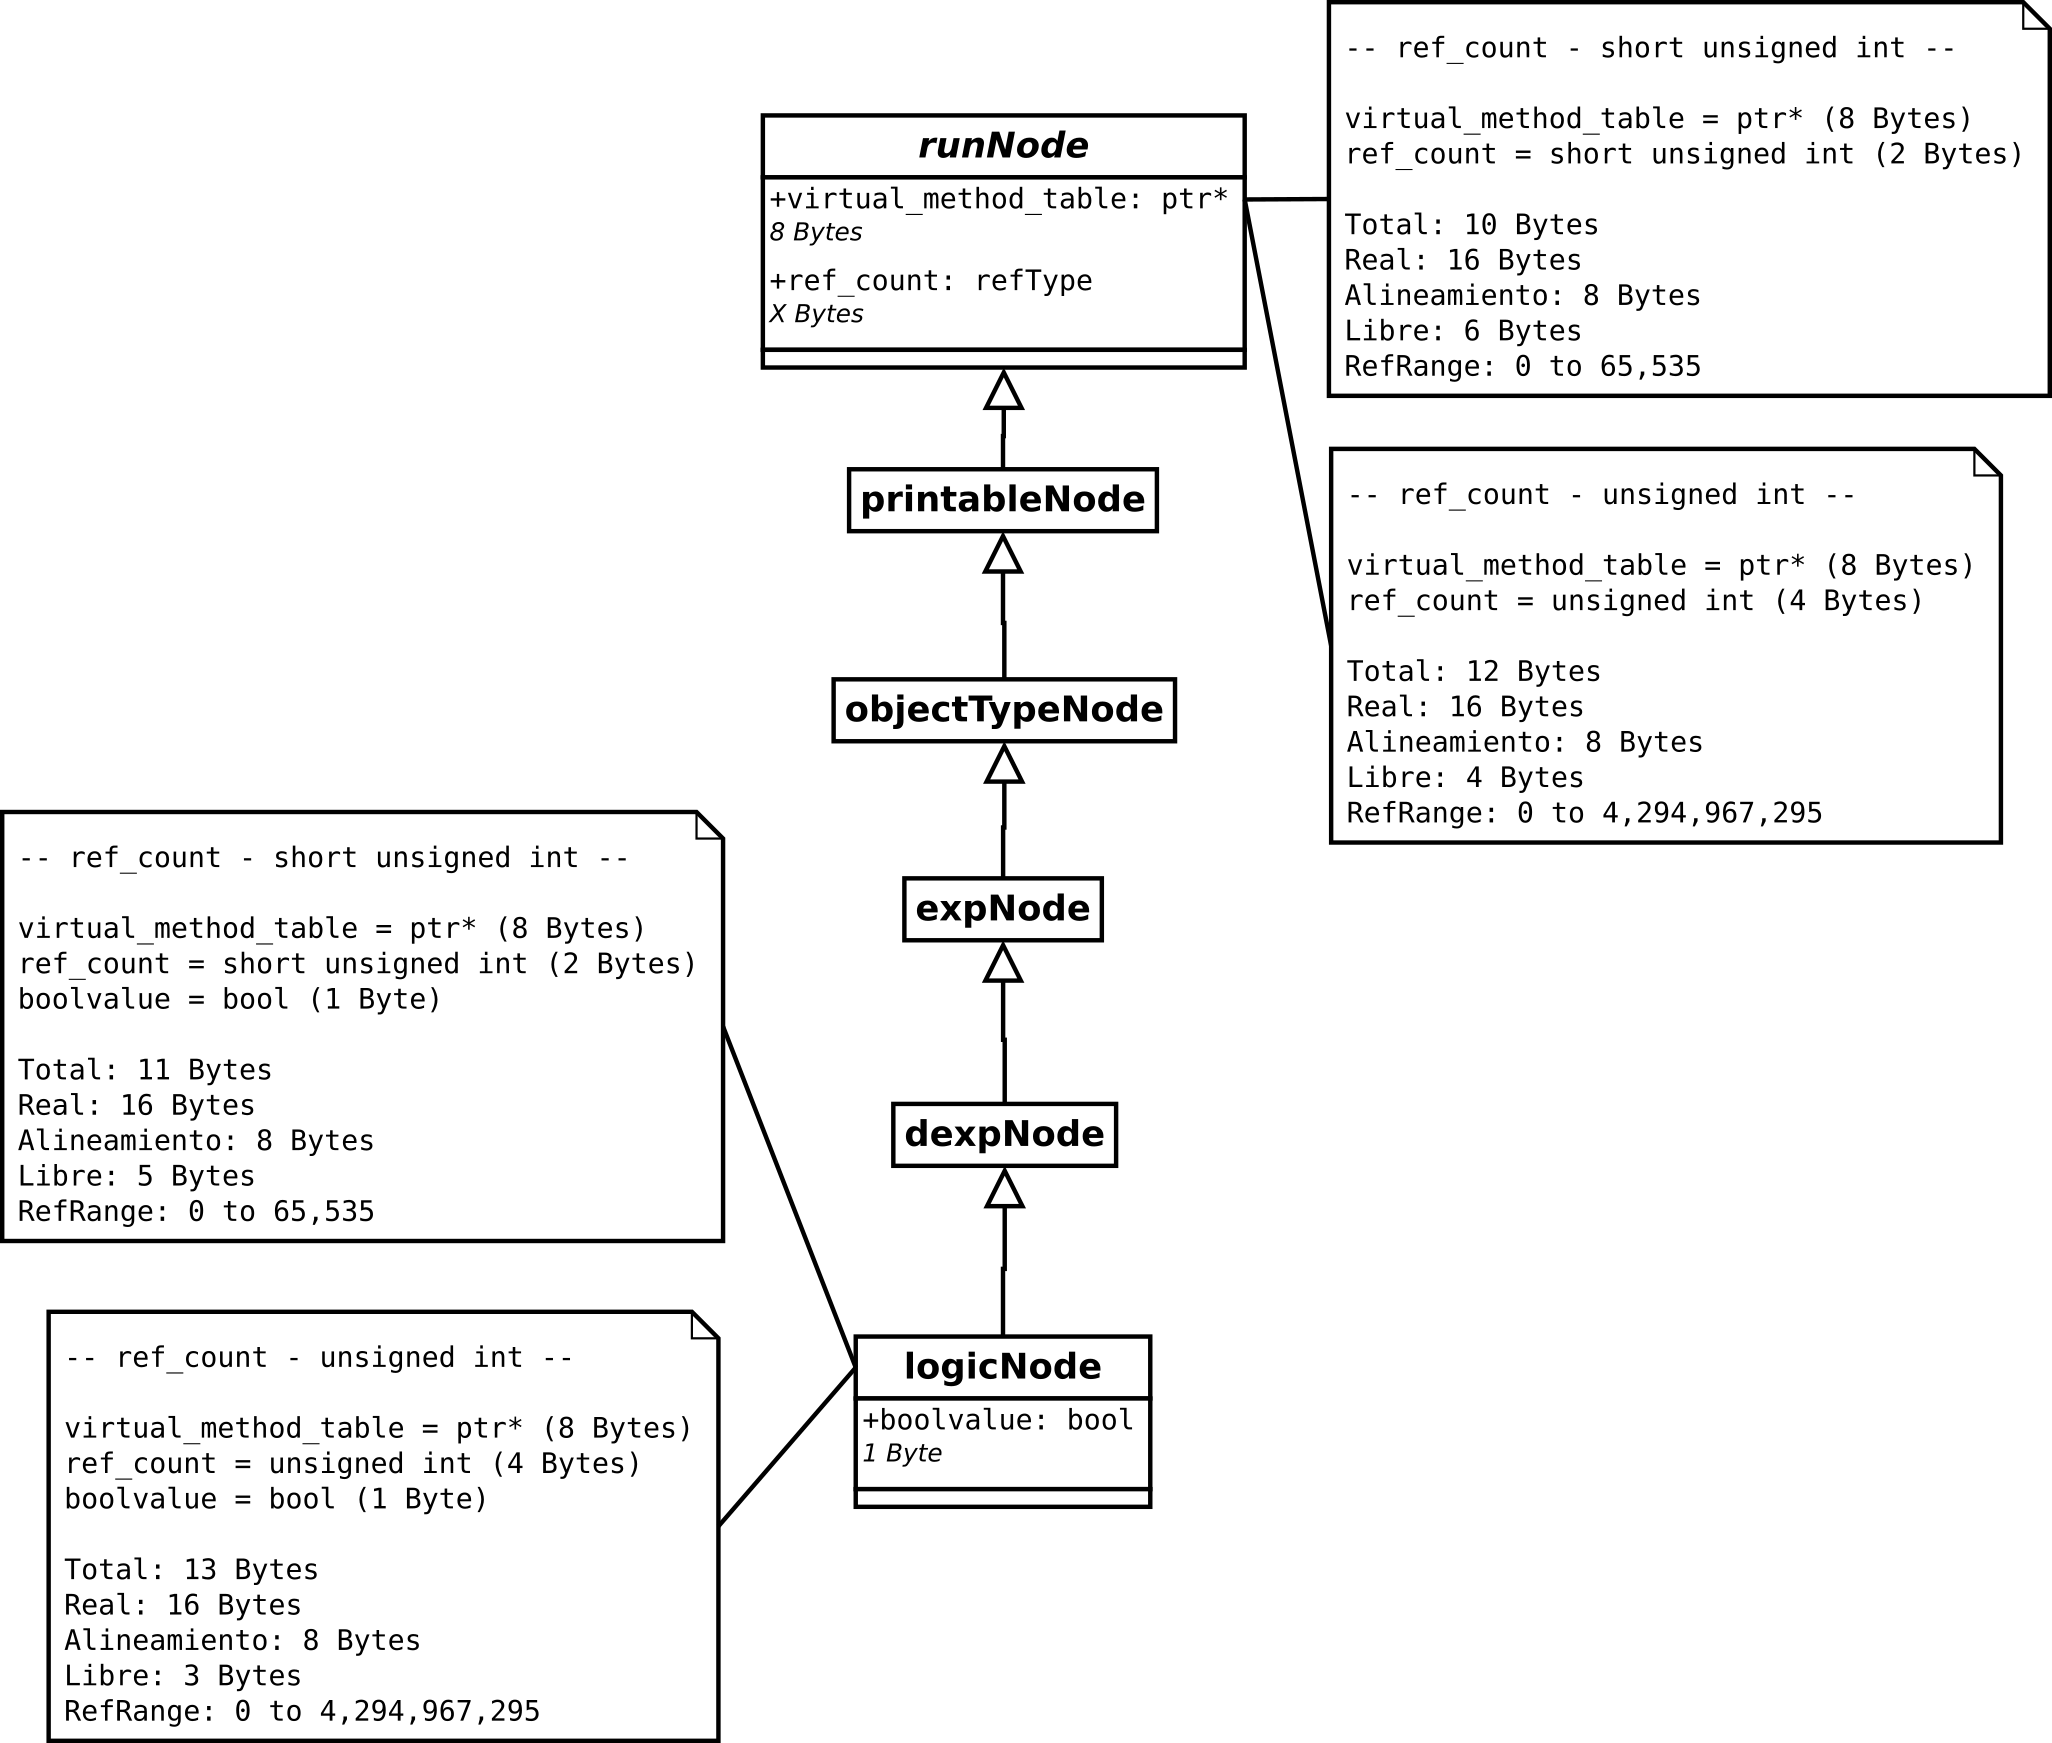
\includegraphics[scale=0.3]{test/memorySpaceLogic.png} 
\captionof{figure}{Espacio de memoria de nodos lógicos}
\end{center}

\pagebreak 
\paragraph{Nodos aritméticos}

En el siguiente diagrama se presenta la memoria ocupada por un nodo de tipo aritmético según las distintas combinaciones para la representación interna de los datos:

\begin{center}
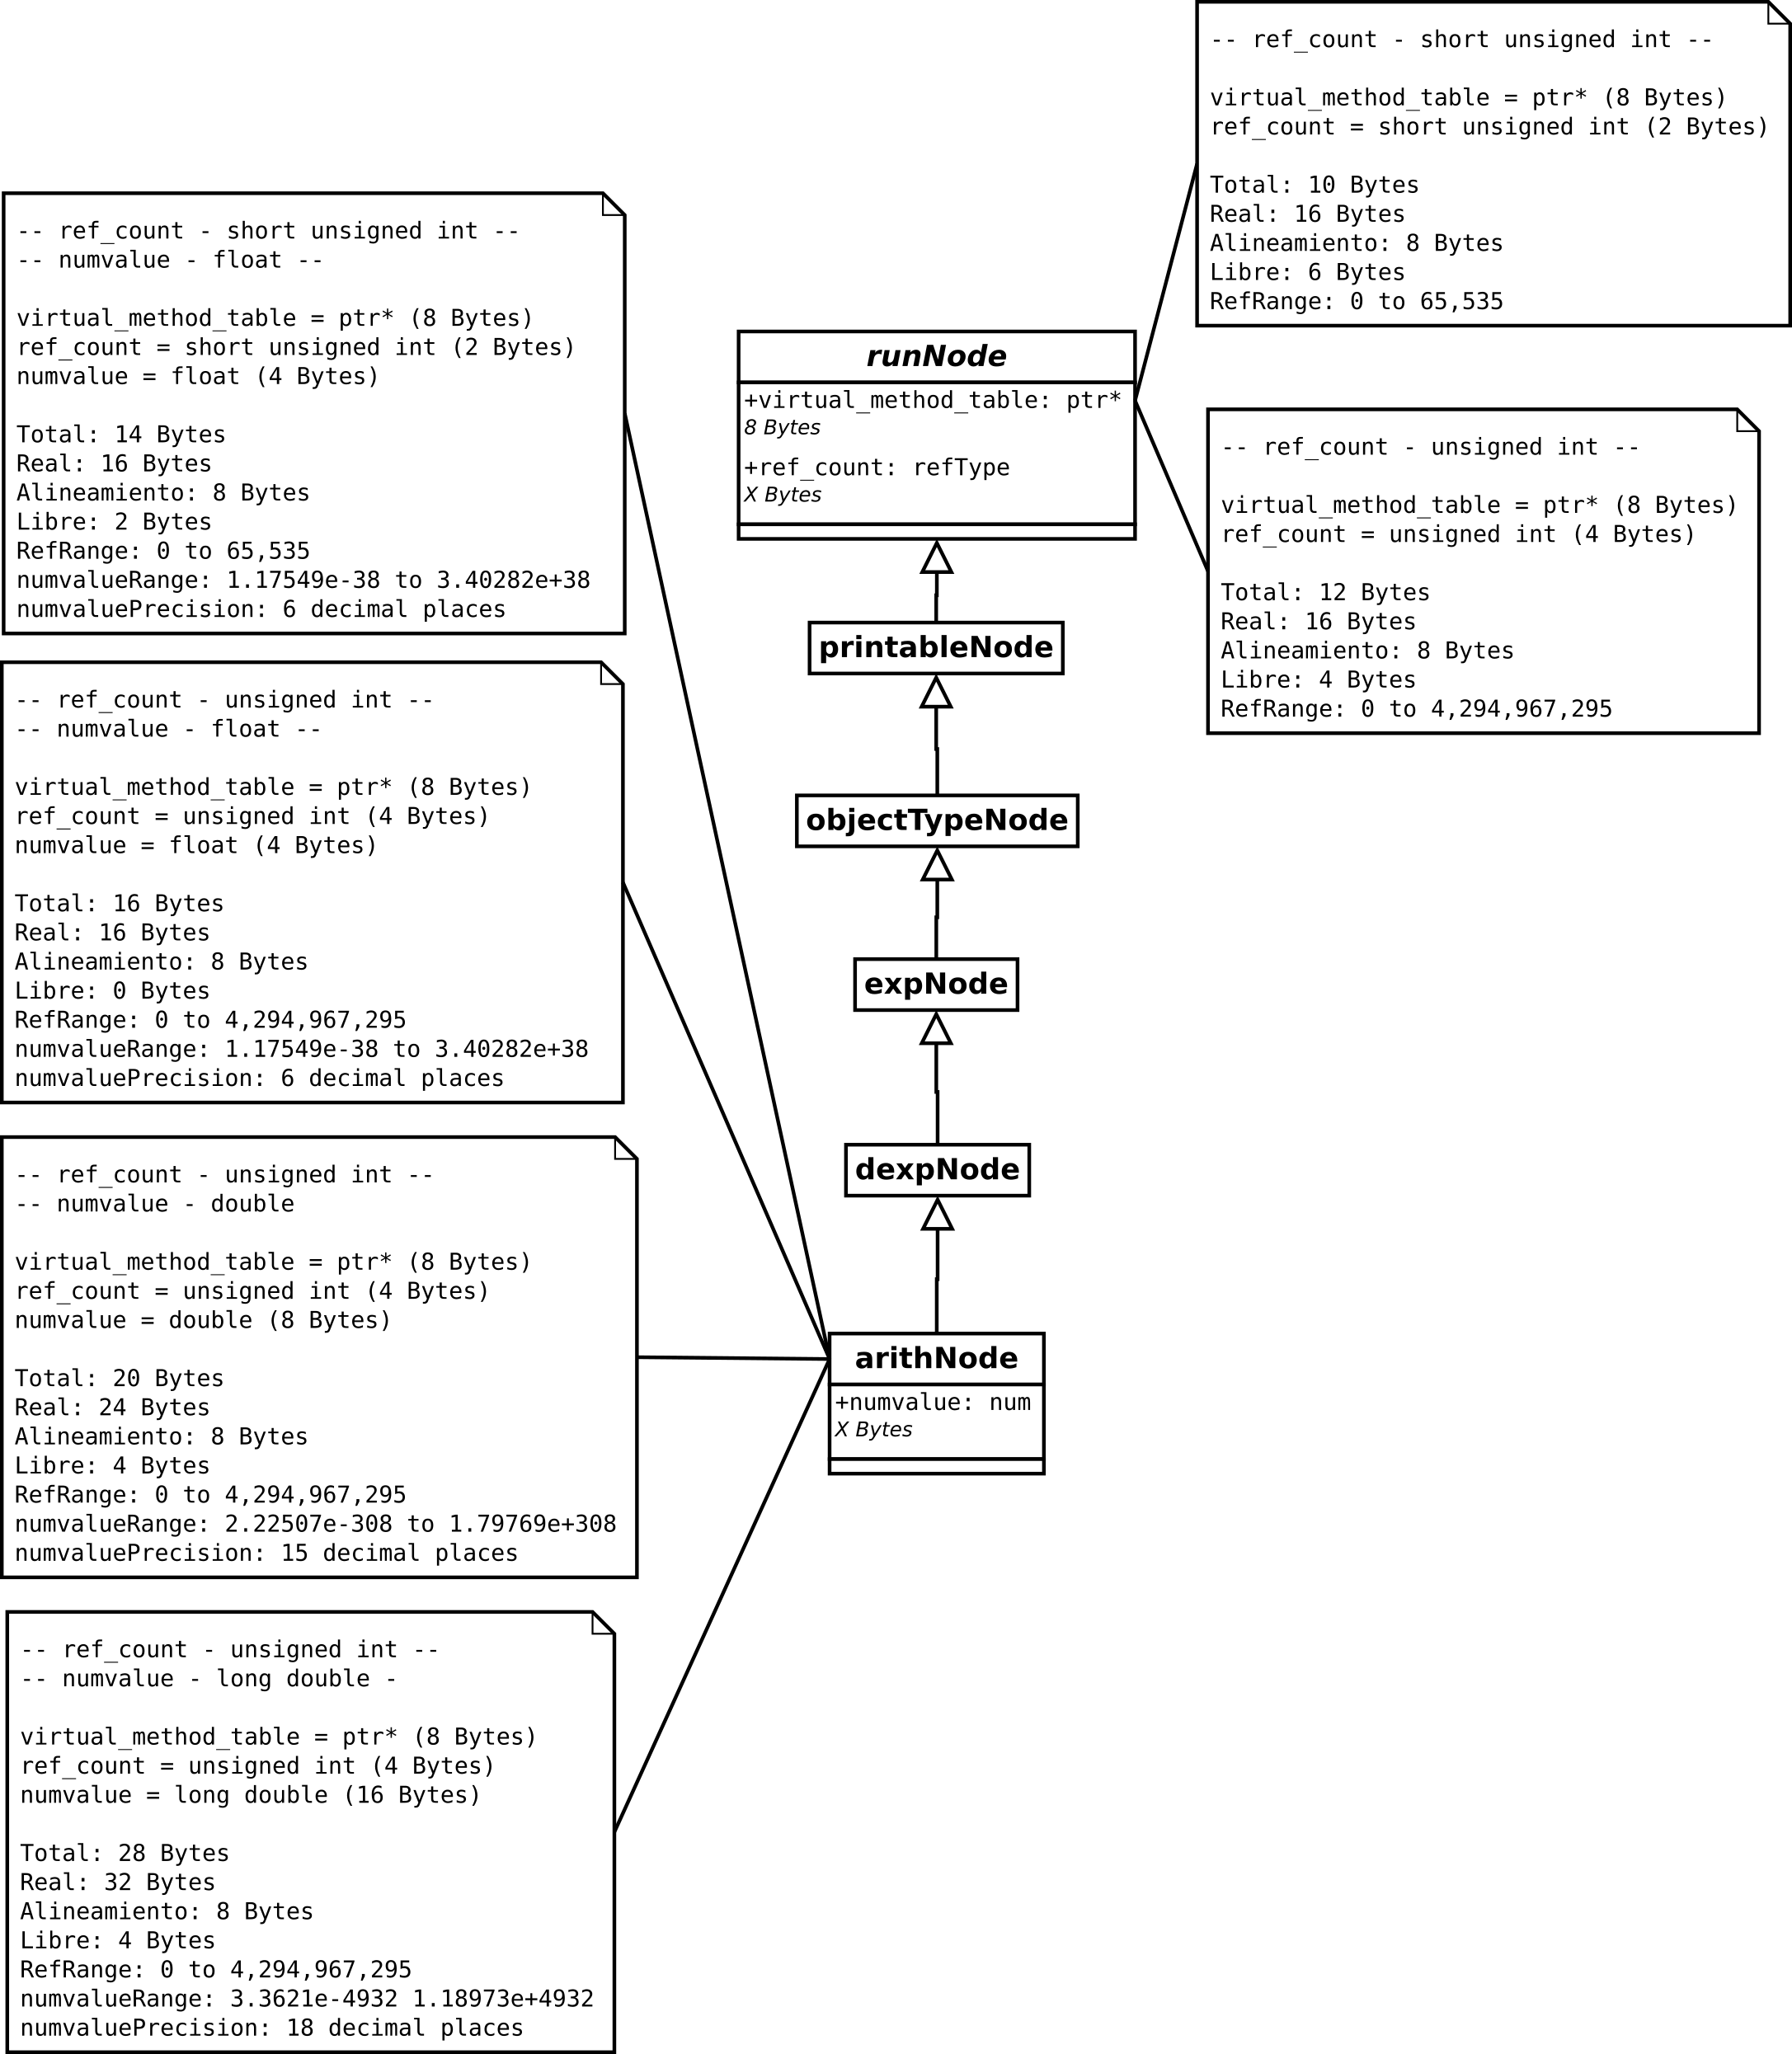
\includegraphics[scale=0.3]{test/memorySpaceArith.png} 
\captionof{figure}{Espacio de memoria de nodos aritméticos}
\end{center}

\pagebreak 
\paragraph{Nodos cadenas de caracteres}

En el siguiente diagrama se presenta la memoria ocupada por un nodo de tipo cadena de caracteres según las distintas combinaciones para la representación interna de los datos:

\begin{center}
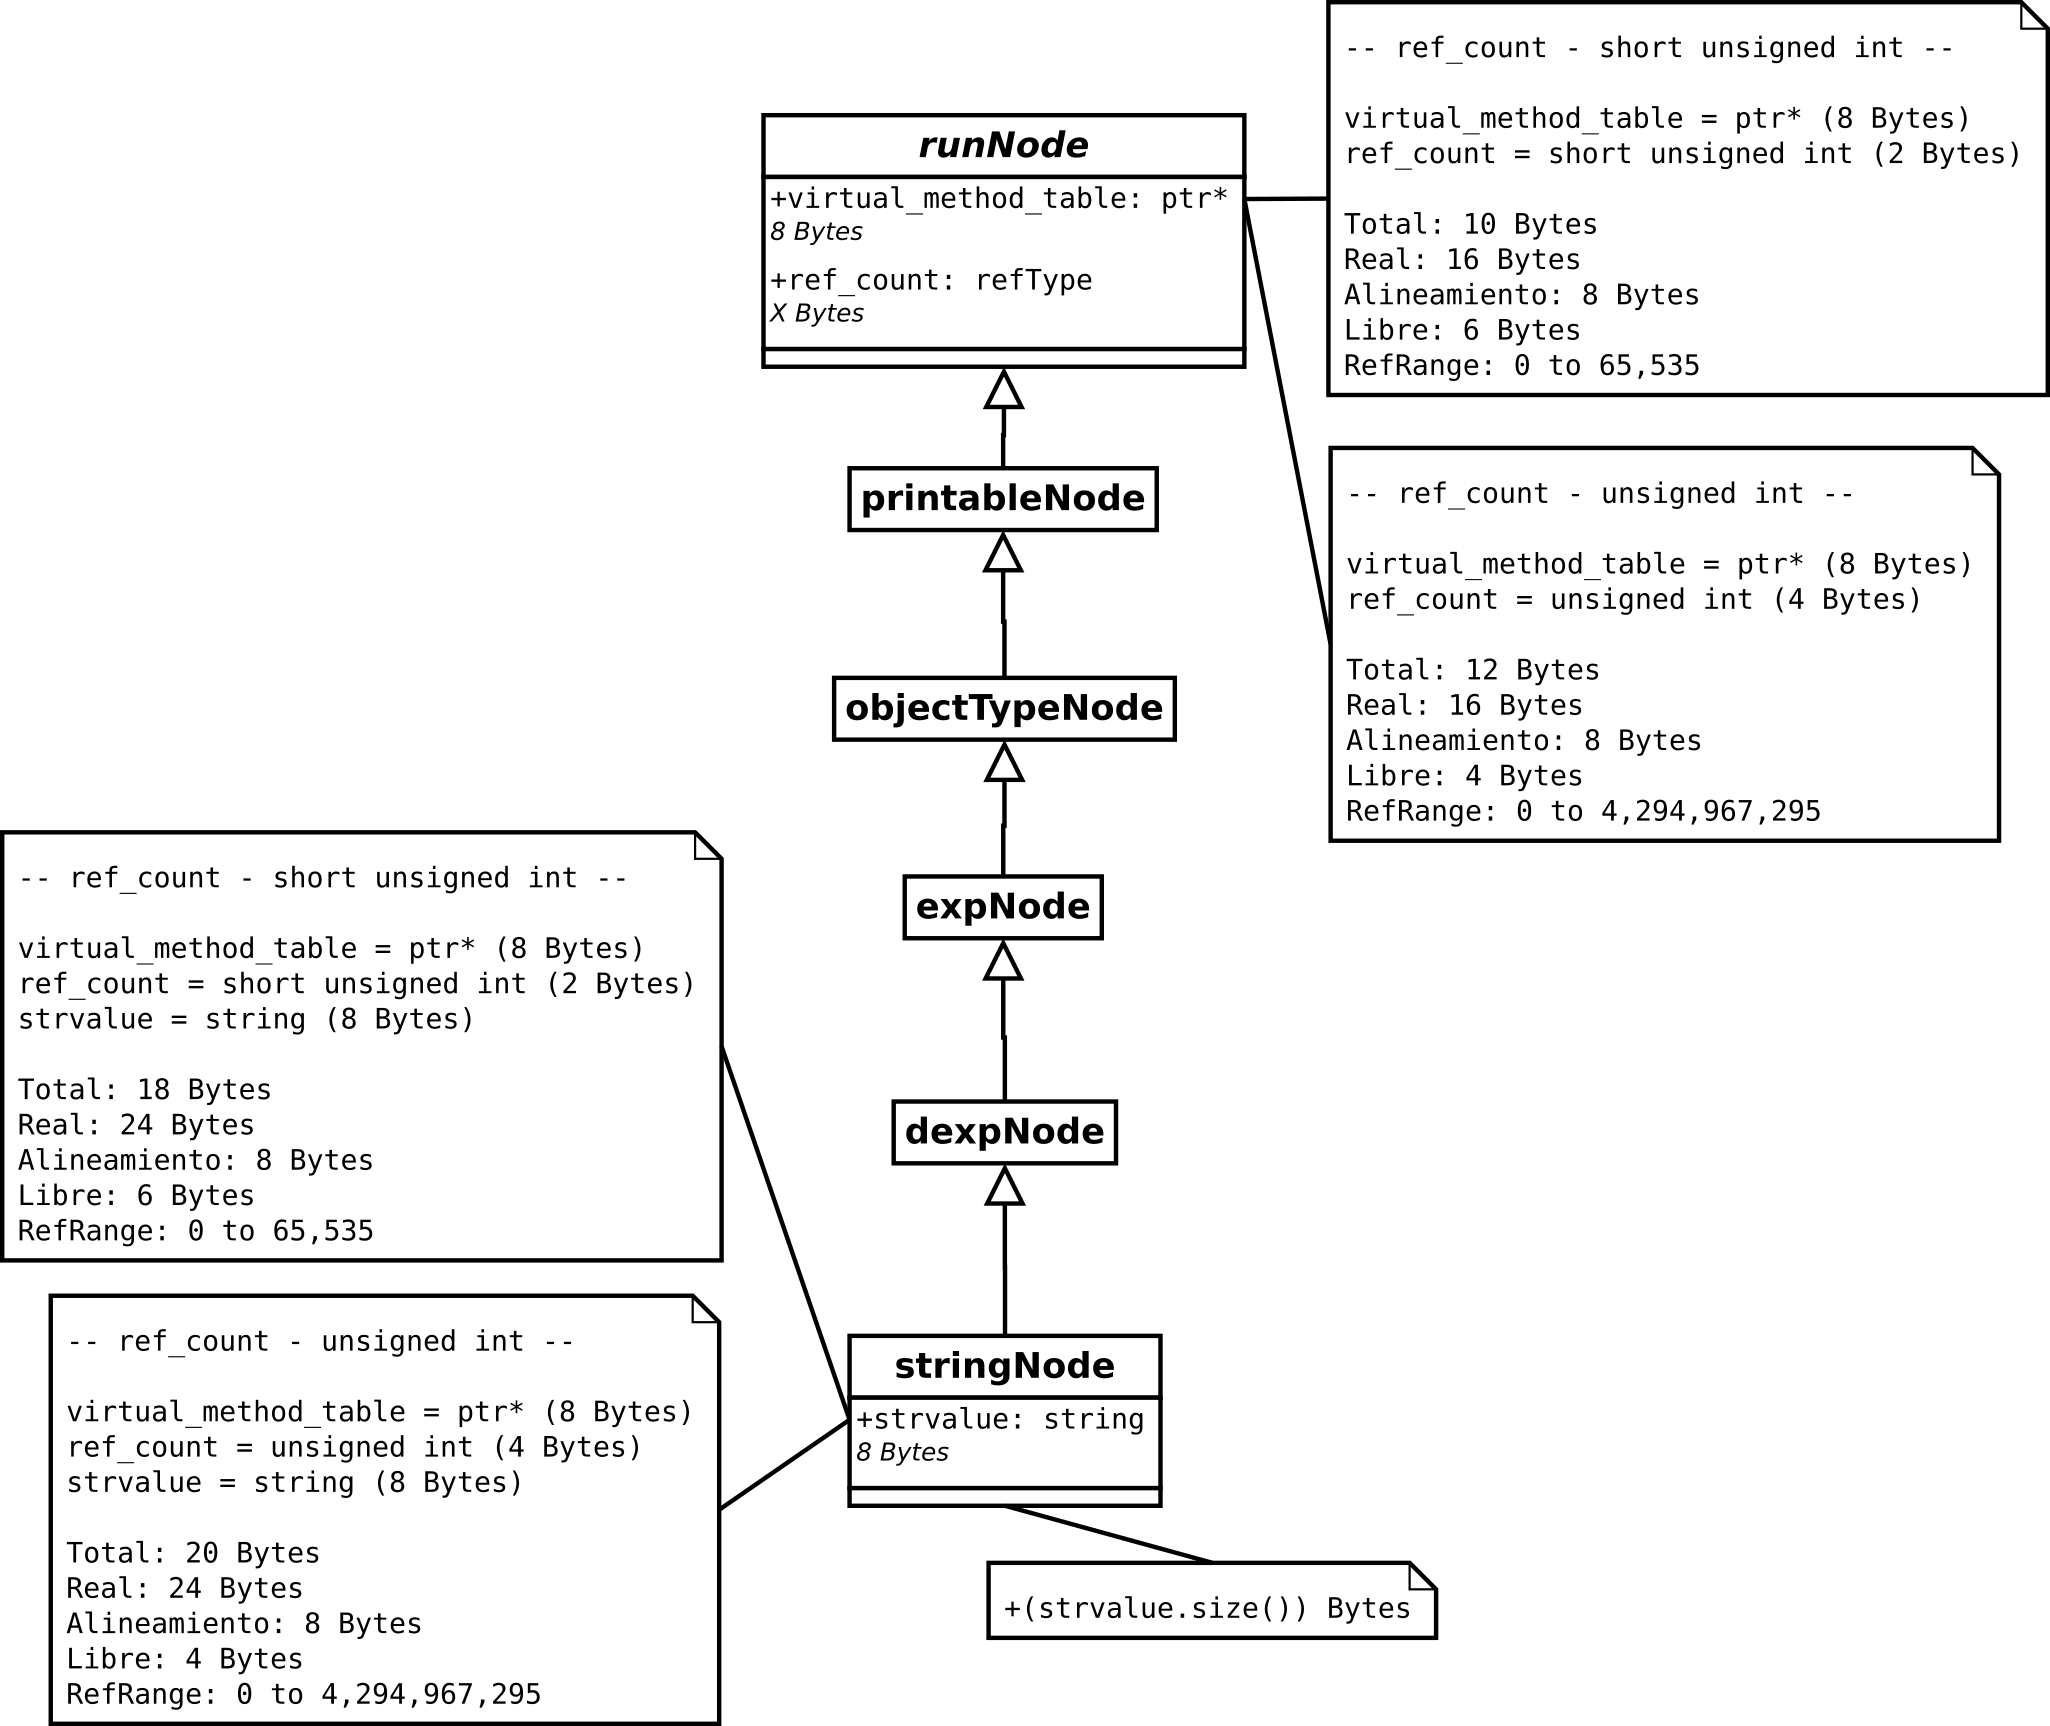
\includegraphics[scale=0.3]{test/memorySpaceStr.png} 
\captionof{figure}{Espacio de memoria de nodos de cadenas de caracteres}
\end{center}

\subsubsection{Seguridad}

El objetivo de
este punto es medir la calidad en función de la seguridad del software desarrollado. Así, para asegurar que la aplicación cumple un mínimo de seguridad se han realizado una serie de 
auditorías al software. 

En el tipo de pruebas realizadas solo se ha tenido en cuenta el software correspondiente al interprete, dejando fuera todo el sistema web que conforma la plataforma de distribución. Un 
sistema web se ve afectado por tipos de vulnerabilidades tales como DoS, XSS, CSRF, SQL injectión, sistemas de autentificación... Por otro lado en un software de escritorio, como 
puede ser el interprete, se ve afectado por otro tipos de vulnerabilidades comunes.

Las pruebas que se han realizado sobre el software se enfocan en la entrada del usuario y se pueden categorizar de la siguiente forma:

\begin{description}
\item[Desbordamiento de buffer:] Se ha comprobado las entradas directas del programa, controlando el tamaño máximo de estas para evitar el desbordamiento de la zona de memoria de datos.
\item[Desbordamiento de buffer por variables de entorno:] Se han controlado el uso de las variables de entorno para que estas no puedan ser usadas para desbordar el espacio de memoria 
destinada a los datos y sobrescribir punteros de control como el de la próxima instrucción.
\item[Inyección de código:] En instrucciones el las que se hace uso de otros lenguajes como por ejemplo para base de datos, se ha comprobado la entrada para que no sea posible modificar la consulta interna.
\item[Salto de directorio:] Se ha comprobado que la inclusión de ficheros no dependa directamente de una entrada sin verificar. Se ha intentado enjaular la aplicación para que no sea posible la 
inclusión de ficheros del sistema por parte del usuario. 
\end{description}

 %~ \FloatBarrier
   %~ \begin{table}[h]
    %~ \begin{center}
   %~ \begin{tabular}{|l|} \hline 
   %~ Desbordamiento de buffer \\ \hline 
   %~ Desbordamiento de buffer por variables de entorno \\ \hline
   %~ Desbordamiento de buffer por recursos binarios \\ \hline 
   %~ Injección de código \\ \hline 
   %~ Salto de directorio (path traversal) \\ \hline 
   %~ \end{tabular}
   %~ \end{center}
   %~ \end{table}
   %~ \FloatBarrier

